%%%%%%%%%%%%%%%%%%%%%%%%%%%%%%%%%%%%%%%%
% Human Genetics Team Talks 
% 30 minute talk on OpenStack and the future of computing at Sanger
% Wellcome Trust Sanger Institute
% 7th October 2016
% Joshua C. Randall
% 
% This work is licensed under the Creative Commons Attribution-ShareAlike 4.0 
% International License. To view a copy of this license, visit 
% http://creativecommons.org/licenses/by-sa/4.0/.
%
% It should be attributed to Joshua C. Randall, Genome Research Limited.
%
% It includes some images which are used under license and which are 
% available separately under their own license terms (all are CC licenses).
% 
% Comments next to each image included in this document cite the source.
% 
%%%%%%%%%%%%%%%%%%%%%%%%%%%%%%%%%%%%%%%%
\documentclass[xcolor=x11names,compress]{beamer}

\usepackage{graphicx}
\DeclareGraphicsExtensions{.pdf,.png,.jpg}
\usepackage{xcolor}
\usepackage{overpic}

% Sanger colour palette
\definecolor{sangerdarkblue}{RGB}{0, 72, 105}
\definecolor{sangermidblue}{RGB}{138, 187, 238}
\definecolor{sangerlightblue1}{RGB}{159, 198, 238}
\definecolor{sangerlightblue2}{RGB}{184, 210, 239}
\definecolor{sangerlightblue3}{RGB}{203, 220, 230}
\definecolor{sangerlightteal}{RGB}{176, 227, 192}
\definecolor{sangerlimegreen}{RGB}{204, 242, 132}
\definecolor{sangerolivegreen}{RGB}{95, 128, 17}
\definecolor{sangerdarkteal}{RGB}{5, 122, 82}
\definecolor{sangermintgreen}{RGB}{221, 246, 164}
\definecolor{sangerdarkbrown}{RGB}{132, 109, 83}
\definecolor{sangerlightbrown}{RGB}{204, 179, 118}
\definecolor{sangerdarkmustard}{RGB}{132, 93, 0}
\definecolor{sangerredbrown}{RGB}{98, 23, 0}
\definecolor{sangerorange}{RGB}{255, 114, 0}
\definecolor{sangerred}{RGB}{195, 0, 29}
\definecolor{sangerdarkred}{RGB}{141, 0, 23}
\definecolor{sangerpurple}{RGB}{124, 0, 79}

% Beamer Layout 
\useoutertheme[subsection=false,shadow]{miniframes}
\useinnertheme{default}
\usefonttheme{serif}
\usepackage{palatino}

\setbeamerfont{title like}{shape=\scshape}
\setbeamerfont{frametitle}{shape=\scshape}

\setbeamercolor*{background canvas}{bg=black}
\setbeamercolor*{lower separation line head}{bg=sangerdarkblue} 
\setbeamercolor*{alerted text}{fg=red} 
\setbeamercolor*{palette tertiary}{fg=black,bg=black!10} 
\setbeamercolor*{palette quaternary}{fg=black,bg=black!10} 

\newcommand{\darkcolors}{
\setbeamercolor*{normal text}{fg=white, bg=black} 
\setbeamercolor*{example text}{fg=white} 
\setbeamercolor*{structure}{fg=sangerlightblue2}  
\setbeamercolor*{frametitle}{fg=sangerlightblue2}  
\setbeamercolor*{itemize/enumerate body}{fg=white}
\setbeamercolor*{itemize/enumerate subbody}{fg=white}
}

\newcommand{\lightcolors}{
\setbeamercolor*{normal text}{fg=black, bg=white} 
\setbeamercolor*{example text}{fg=black} 
\setbeamercolor*{structure}{fg=sangerdarkblue} 
\setbeamercolor*{frametitle}{fg=black} 
\setbeamercolor*{itemize/enumerate body}{fg=black}
\setbeamercolor*{itemize/enumerate subbody}{fg=black}
}

\darkcolors

\renewcommand{\(}{\begin{columns}}
\renewcommand{\)}{\end{columns}}
\newcommand{\<}[1]{\begin{column}{#1}}
\renewcommand{\>}{\end{column}}

% title page colours
\newcommand{\titlepagefgcolour}{white}
\setbeamercolor*{title}{fg=\titlepagefgcolour}
\setbeamercolor*{subtitle}{fg=\titlepagefgcolour}
\setbeamercolor*{author}{fg=\titlepagefgcolour}
\setbeamercolor*{institute}{fg=\titlepagefgcolour}
\setbeamercolor*{date}{fg=\titlepagefgcolour}


% backgroundblock environment for background images
% from: "beamer: How to place images behind text (z-order)"
% (http://tex.stackexchange.com/a/134311)
\makeatletter
\newbox\@backgroundblock
\newenvironment{backgroundblock}[2]{%
  \global\setbox\@backgroundblock=\vbox\bgroup%
    \unvbox\@backgroundblock%
    \vbox to0pt\bgroup\vskip#2\hbox to0pt\bgroup\hskip#1\relax%
}{\egroup\egroup\egroup}
\addtobeamertemplate{background}{\box\@backgroundblock}{}
\makeatother

% setup shadedbox environment as an mdframed box with partial opacity
\usepackage[framemethod=tikz]{mdframed}
\newmdenv[tikzsetting={draw=none,fill=black,fill opacity=0.5},backgroundcolor=none]{shadedbox}

\begin{document}

% background shading overlay
\newcommand{\shadedbackground}[2]{
	\begin{backgroundblock}{-2pt}{-2pt}
		\vbox to #2\paperheight{\vfil\hbox to \paperwidth{\hfil
		\begin{tikzpicture}
		\fill[black,opacity=#1] (0,0) rectangle (\paperwidth,#2\paperheight);
		\end{tikzpicture}
		\hfil\hskip 2mm}\vfil}
	\end{backgroundblock}
}

% white background: \whitebackground{opacity}{height}{y}
\newcommand{\whitebackground}[3]{
	\begin{backgroundblock}{0cm}{0cm}
		\vbox to \paperheight{\vfil\hbox to \paperwidth{\hfil
		\begin{tikzpicture}
		\fill[white,opacity=#1] (0,#3\paperheight) rectangle (\paperwidth,#2\paperheight);
		\end{tikzpicture}
		\hfil\hskip 2mm}\vfil}
	\end{backgroundblock}
}
% pipework background image
\newcommand{\pipesbackground}{
	\begin{backgroundblock}{0cm}{0cm}
		\vbox to \paperheight{\vfil\hbox to \paperwidth{\hfil
		\begin{overpic}[grid=false,height=0.85\paperheight]{images/Jano_De_Cesare_-_Pipelines_-_by-nc-nd-2_0_-_flickr}
		% Image source: https://www.flickr.com/photos/janodecesare/3020406104/
		\put(88,0.5){\textcolor{gray}{\fontsize{4}{6}\selectfont Photo: Jano De Cesare}}
		\end{overpic}
		\hfil\hskip 2mm}\vfil}
	\end{backgroundblock}
}


% Sanger Data Centre background image
\newcommand{\dcbackground}{
	\begin{backgroundblock}{0cm}{0cm}
		\vbox to \paperheight{\vfil\hbox to \paperwidth{\hfil
		\begin{overpic}[grid=false,height=0.85\paperheight]{images/Sanger_-_data_centre_80-1300px_-_by-3_0_-_GRL}
		% Image source: http://www.sanger.ac.uk/sites/default/files/styles/slider_1268_610/public/data_centre_80-1300px.jpg
		\put(88,0.5){\textcolor{gray}{\fontsize{4}{6}\selectfont Photo: Genome Research Limited}}	
		\end{overpic}
		\hfil\hskip 2mm}\vfil}
	\end{backgroundblock}
}

% Sanger Data Centre background image with rays
\newcommand{\dcraysbackground}{
	\begin{backgroundblock}{0cm}{0cm}
		\vbox to \paperheight{\vfil\hbox to \paperwidth{\hfil
		\hspace{-4cm}\begin{overpic}[grid=false,height=0.85\paperheight]{images/Sanger_-_data_centre_34-1300px_1_-_by-3_0_-_GRL}
		% Image source: http://www.sanger.ac.uk/sites/default/files/styles/slider_1268_610/public/data_centre_34-1300px_1.jpg
		\put(88,0.5){\textcolor{gray}{\fontsize{4}{6}\selectfont Photo: Genome Research Limited}}	
		\end{overpic}
		\hfil\hskip 2mm}\vfil}
	\end{backgroundblock}
}

% Sequencing background image
\newcommand{\seqbackground}{
	\begin{backgroundblock}{0cm}{0cm}
		\vbox to \paperheight{\vfil\hbox to \paperwidth{\hfil
		\begin{overpic}[grid=false,height=0.85\paperheight]{images/Sanger_-_sequencers_1495-1300px_-_by-3_0_-_GRL}
		% Image source: http://www.sanger.ac.uk/sites/default/files/styles/slider_1268_610/public/_1495-1300px.jpg
		\put(88,0.5){\textcolor{gray}{\fontsize{4}{6}\selectfont Photo: Genome Research Limited}}	
		\end{overpic}
		\hfil\hskip 2mm}\vfil}
	\end{backgroundblock}
}

% Clouds background image
\newcommand{\cloudsbackground}{
	\begin{backgroundblock}{-2pt}{-2pt}
		\vbox to \paperheight{\vfil\hbox to \paperwidth{\hfil
		\begin{overpic}[grid=false,height=0.85\paperheight]{images/Keith_Pomakis_-_Cumulus_Clouds_Over_Jamaica_-_cc-by-sa-2_5_-_wikimedia_-_cropped}
		% Image source: https://commons.wikimedia.org/wiki/File:Cumulus_Clouds_Over_Jamaica.jpg
		\put(88,0.5){\textcolor{gray}{\fontsize{4}{6}\selectfont Photo: Keith Pomakis}}
		\end{overpic}
		\hfil\hskip 2mm}\vfil}
	\end{backgroundblock}
}


%%%%%%%%%%%%%%%%%%%%%%%%%%%%%%%%%%%%%%%%
% Introduction
%%%%%%%%%%%%%%%%%%%%%%%%%%%%%%%%%%%%%%%%
\section*{\scshape Introduction}
\begin{frame}
\title{OpenStack and the future of scientific computing at the Sanger Institute}
\author{
	Joshua C. Randall \\
	{\it 
	Human Genetics Informatics \\
	Wellcome Trust Sanger Institute 
	}\\
}
\date{
	% HGI logo is covered under the license for this work
	\scalebox{0.5}{
\includegraphics{images/HGI-ltblue}} \\
	\vspace{0.5cm}
	7th October 2016
}
%\dcbackground
\titlepage
\end{frame}

% HGI logo in bottom left corner of remaining frames
\addtobeamertemplate{background}{\vbox to0pt{\vskip 8.9cm \hbox to0pt{\hskip 1mm \relax
	% HGI logo is covered under the license for this work
	
\includegraphics[height=0.6cm]{images/HGI-ltblue}
}}}

%%%%%%%%%%%%%%%%%%%%%%%%%%%%%%%%%%%%%%%%
% Table of Contents
%%%%%%%%%%%%%%%%%%%%%%%%%%%%%%%%%%%%%%%%
%\begin{frame}{Introduction}
%\dcbackground
%\begin{shadedbox}
%\tableofcontents
%\end{shadedbox}
%\end{frame}

%%%%%%%%%%%%%%%%%%%%%%%%%%%%%%%%%%%%%%%%
% The farm
%%%%%%%%%%%%%%%%%%%%%%%%%%%%%%%%%%%%%%%%
\section{\scshape The farm}

%%%%%%%%%%%%%%%%%%%%%%%%%%%%%%%%%%%%%%%%
\begin{frame}{The farm}
\dcbackground
\shadedbackground{0.5}{1}
\begin{backgroundblock}{0cm}{0cm}
		\vbox to \paperheight{\vfil\hbox to \paperwidth{\hskip 0.025\paperwidth 
		\begin{overpic}[width=0.95\paperwidth]{images/sanger-farm3-2016-diagram}
		% Diagram: drawn by Joshua C. Randall, GRL
		\end{overpic}
		\hfil\hskip 2mm}\vfil}
\end{backgroundblock}
\end{frame}

%%%%%%%%%%%%%%%%%%%%%%%%%%%%%%%%%%%%%%%%
\subsection*{The farm is old technology}
\begin{frame}{The farm is old technology}
\dcbackground
\begin{backgroundblock}{0cm}{0cm}
		\vbox to \paperheight{\vfil\hbox to \paperwidth{\hskip 7.8cm 
		\begin{overpic}[width=0.35\paperwidth]{images/utopia-lsf-title-april-1992}
		% Image source: doi:10.1.1.121.1434
		\end{overpic}
		\hfil\hskip 2mm}\vfil}
\end{backgroundblock}
\begin{shadedbox}[rightmargin=0.35\paperwidth]
\begin{itemize}
\item Basic architecture unchanged for 30+ years % (cluster compute with shared network storage)
\item LSF developed 25 years ago
\item OS on farm3 is 4.5 years old
\item Change happens infrequently
	\begin{itemize}
	\item Expensive for sysadmins
	\item Painful for users
	\end{itemize}
\end{itemize}
\end{shadedbox}
\end{frame}

%%%%%%%%%%%%%%%%%%%%%%%%%%%%%%%%%%%%%%%%
\subsection*{The farm is difficult to scale}
\begin{frame}{The farm is difficult to scale}
\dcbackground
\shadedbackground{0.5}{1}
\begin{backgroundblock}{0cm}{0cm}
		\vbox to \paperheight{\vfil\hbox to \paperwidth{\hskip 0.025\paperwidth 
		\begin{overpic}[width=0.95\paperwidth]{images/sanger-farm3-2016-diagram}
		% Diagram: drawn by Joshua C. Randall, GRL
		\end{overpic}
		\hfil\hskip 2mm}\vfil}
\end{backgroundblock}
\end{frame}

%%%%%%%%%%%%%%%%%%%%%%%%%%%%%%%%%%%%%%%%
\subsection*{The farm is heterogeneous}
\begin{frame}{The farm is heterogeneous}
\dcbackground
\begin{shadedbox}[leftmargin=0,rightmargin=0]
\begin{itemize}
\item 52 different software configurations across 297 compute nodes on farm3
\end{itemize}
{\color{white}\setlength{\tabcolsep}{4pt}
	\begin{tabular}{ p{4em} | c c c c c c c c c c c c c c }
		& & & & & & & & & & & & & \\
		Configs & 34 & 5 & 1 & 2 & 1 & 1 & 1 & 1 & 1 & 1 & 1 & 1 & 1 & 1 \\
		\hline
		Nodes & 1 & 2 & 3 & 7 & 8 & 10 & 14 & 18 & 20 & 26 & 30 & 32 & 37 & 41 \\
	\end{tabular}
	}
\end{shadedbox}
\end{frame}

%%%%%%%%%%%%%%%%%%%%%%%%%%%%%%%%%%%%%%%%
\subsection*{The farm is hard to use}
\begin{frame}{The farm is hard to use}
\dcbackground
\begin{shadedbox}[leftmargin=0,rightmargin=0]
\begin{itemize}
\item User interface is low-level and difficult to use
	\begin{itemize}
	\item Most power users end up writing code or using external systems to manage their work
	\item LSF CLI is inconsistent and output is difficult to parse
	\item Documentation is poor, encourages trial \& error
	\end{itemize}
\item Components fail often, but software does little to help manage failure
	\begin{itemize}
	\item Users just want to get their work done
	\item End up spending a lot of time fighting with job failures
	\end{itemize}
\item Scheduler is hard-coded to obsess about core hours,
	\begin{itemize}
	\item Often memory or I/O are the real contended resources
	\item Some users are rewarded for effort spent gaming the system
	\end{itemize}
\end{itemize}
\end{shadedbox}
\end{frame}

%%%%%%%%%%%%%%%%%%%%%%%%%%%%%%%%%%%%%%%%
\subsection*{The farm is wasteful}
\begin{frame}{The farm is wasteful}
\dcbackground
\begin{shadedbox}
\begin{itemize}
\item LSF scheduler doesn't optimise resource utilisation very well
\item Multiple isolated clusters that can't share resource
	\begin{itemize}
	\item farm3, vr-farm, cgp-farm, 
	\end{itemize}
\end{itemize}
\end{shadedbox}
\end{frame}

%%%%%%%%%%%%%%%%%%%%%%%%%%%%%%%%%%%%%%%%
\subsection*{The farm is dead}
\begin{frame}{The farm is dead}
\dcbackground
\begin{shadedbox}
\begin{itemize}
\item No new hardware will be bought for farm3
	\begin{itemize}
	\item Informatics Committee decision as of mid 2016
	\end{itemize}
\item EOL for farm3 OS (Ubuntu 12.04 LTS): October 2017
\item No plan for general purpose replacement % ``farm4''
	\begin{itemize}
	\item Don't expect a farm3 $\rightarrow$ farm4 transition %as happened with farm2 $\rightarrow$ farm3
	\end{itemize}
\end{itemize}
\end{shadedbox}
\end{frame}


\begin{frame}{The farm is dead}
\dcbackground
\shadedbackground{0.5}{1}
\begin{backgroundblock}{0cm}{0cm}
		\vbox to \paperheight{\vfil\hbox to \paperwidth{\hskip 0.025\paperwidth 
		\begin{overpic}[width=0.95\paperwidth]{images/sanger-farm3-2016-diagram}
		% Diagram: drawn by Joshua C. Randall, GRL
		\end{overpic}
		\hfil\hskip 2mm}\vfil}
\end{backgroundblock}
\end{frame}


%%%%%%%%%%%%%%%%%%%%%%%%%%%%%%%%%%%%%%%%
\subsection*{Long live the farm}
\begin{frame}{Long live the farm}
\dcbackground
\begin{backgroundblock}{0cm}{0cm}
		\vbox to \paperheight{\vfil\hbox to \paperwidth{\hskip 0.025\paperwidth 
		\begin{overpic}[width=0.95\paperwidth]{images/sanger-farm3-2016-diagram}
		% Diagram: drawn by Joshua C. Randall, GRL
		\end{overpic}
		\hfil\hskip 2mm}\vfil}
\end{backgroundblock}
\shadedbackground{0.75}{1}
\begin{shadedbox}
\begin{itemize}
\item The farm handles most scientific computing workloads today
		\begin{itemize}
		\item 72M core-hours reserved last year across institute % $\sim$
		\item humgen reserved 25M core-hours last year
		\item humgen used 10M core-hours last year
		\end{itemize}
\item Users (and scripts) expect LSF commands
		\begin{itemize}
		\item bsub, bjobs, bqueues, etc...
		\end{itemize}
\item LSF license \& support committment for 3+ years
		\begin{itemize}
		\item Current hardware will be retired instead of replaced
		\item Virtual LSF clusters can replace them as needed
		\end{itemize}
\end{itemize}
\end{shadedbox}
\end{frame}


\section[\scshape OpenStack IaaS]{\scshape OpenStack Infrastructure-as-a-Service}
%%%%%%%%%%%%%%%%%%%%%%%%%%%%%%%%%%%%%%%%
\subsection*{OpenStack Infrastructure-as-a-Service (IaaS)}
\begin{frame}{OpenStack Infrastructure-as-a-Service (IaaS)}
\dcbackground
\shadedbackground{0.5}{1}
\begin{backgroundblock}{0cm}{0cm}
		\vbox to \paperheight{\vfil\hbox to \paperwidth{\hskip 0.075\paperwidth 
		\begin{overpic}[width=0.85\paperwidth]{images/OpenStack-installguidearch-neutron-hw_-_OpenStack_Foundation_-_Apache_2_0_-_cropped}
		% Image: OpenStack Foundation, Apache 2.0 license
		\end{overpic}
		\hfil\hskip 2mm}\vfil}
\end{backgroundblock}
\end{frame}

\lightcolors

%%%%%%%%%%%%%%%%%%%%%%%%%%%%%%%%%%%%%%%%
\subsection*{OpenStack Services}
\begin{frame}{OpenStack Services}
\cloudsbackground
%\shadedbackground{0.25}{1}
\begin{backgroundblock}{0cm}{0cm}
		\vbox to \paperheight{\vfil\hbox to \paperwidth{\hskip 0.05\paperwidth 
		\begin{overpic}[width=0.9\paperwidth]{images/OpenStack-installguidearch-neutron-services_-_OpenStack_Foundation_-_Apache_2_0_-_cropped}
		% Image: OpenStack Foundation, Apache 2.0 license
		\end{overpic}
		\hfil\hskip 2mm}\vfil}
\end{backgroundblock}
\end{frame}

%%%%%%%%%%%%%%%%%%%%%%%%%%%%%%%%%%%%%%%%
\subsection*{Why OpenStack?}
\begin{frame}{Why OpenStack?}
\cloudsbackground
%\shadedbackground{0.25}{1}
\begin{itemize}
\item Separates responsibility for hardware management from platform \& application-level management
\item Same model as public ``cloud computing''
		\begin{itemize}
		\item Amazon EC2, Google Compute Engine, Rackspace, etc.
		\end{itemize}
\item Programmatic control over:
		\begin{itemize}
		\item Compute instances
		\item Storage
		\item Network connectivity
		\end{itemize}
\item Legacy systems can be redeployed onto OpenStack
	\begin{itemize}
	\item improved consistency
	\item less wasteful
	\item dynamically scalable
	\end{itemize}
\item Empowers users to deploy virtually any system that can run on general purpose computers
\end{itemize}
\end{frame}

%%%%%%%%%%%%%%%%%%%%%%%%%%%%%%%%%%%%%%%%
\subsection*{When will OpenStack be available?}
\begin{frame}{When will OpenStack be available?}
\cloudsbackground
%\shadedbackground{0.25}{1}
\begin{itemize}
\item OpenStack ``SciaaS'' system available to external customers
\item OpenStack-gamma available for internal testing
\item First batch of internal SciaaS hardware has been purchased (\pounds 1.2M)
	\begin{itemize}
	\item Ordered in August 2016
	\item Arrived on campus at the end of September 2016
	\item Currently being commissioned and tested by systems
	\end{itemize}
\item SciaaS production OpenStack system expected to be available in early 2017
\end{itemize}
\end{frame}

\darkcolors

\section{\scshape Tools, Frameworks, \& Platforms}
%%%%%%%%%%%%%%%%%%%%%%%%%%%%%%%%%%%%%%%%
\subsection*{Low-level cluster management}
\begin{frame}{Low-level cluster management}
\pipesbackground
\shadedbackground{0.5}{1}
\begin{itemize}
	\item IBM/Platform LSF (at least for a few more years)
	\item DC/OS
	\item Mesos
	\item Oracle Grid Engine / Sun Grid Engine (SGE)
	\item Simple Linux Utility for Resource Management (SLURM)
\end{itemize}
\end{frame}

%%%%%%%%%%%%%%%%%%%%%%%%%%%%%%%%%%%%%%%%
\subsection*{Long-running service platforms}
\begin{frame}{Long-running service platforms}
\pipesbackground
\shadedbackground{0.5}{1}
\begin{itemize}
	\item Cloud Foundry
	\item Fleet
	\item Kubernetes
	\item Marathon
	\item Swarm
\end{itemize}
\end{frame}

%%%%%%%%%%%%%%%%%%%%%%%%%%%%%%%%%%%%%%%%
\subsection*{High-level workflow management}
\begin{frame}{High-level workflow management}
\pipesbackground
\shadedbackground{0.5}{1}
\begin{itemize}
	\item Arvados (Python, Perl, Ruby, Java, Go, CLI, CWL)
	\item eHive (Perl)
	\item Pegasus (Java, Perl, Python, DAX)
	\item Runner.pm (Perl)
	\item Shock/AWE (CWL)
	\item Taverna (SCUFL2, CWL planned)
	\item Toil (Python, CWL)
	\item VR-Pipe (Perl, CWL planned)
\end{itemize}
\end{frame}

%%%%%%%%%%%%%%%%%%%%%%%%%%%%%%%%%%%%%%%%
\subsection*{Distributed data processing frameworks}
\begin{frame}{Distributed data processing frameworks}
\pipesbackground
\shadedbackground{0.5}{1}
\begin{itemize}
	\item Hadoop (Java, Python)
	\item Hive (HiveQL)
	\item Pig (Pig Latin; extensions in Java, Python, JavaScript, Ruby, or Groovy)
	\item Spark (Java, Scala, Python, R)
\end{itemize}
\end{frame}

%%%%%%%%%%%%%%%%%%%%%%%%%%%%%%%%%%%%%%%%
\subsection*{Interactive platforms}
\begin{frame}{Interactive platforms}
\pipesbackground
\shadedbackground{0.5}{1}
\begin{itemize}
	\item Galaxy Project
	\begin{itemize}
	\item Traditional web interface
	\item Many built-in bioinformatics processes and workflows
	\end{itemize}
	\item Jupyter Notebook
	\begin{itemize}
	\item General purpose interactive web application for developing and sharing code and scripts in many languages
	\item Python
	\item R
	\item Spark
	\item 40+ others
	\end{itemize}
\end{itemize}
\end{frame}


%%%%%%%%%%%%%%%%%%%%%%%%%%%%%%%%%%%%%%%%%
%\subsection*{Apache Spark}
%\darkcolors
%\begin{frame}{Apache Spark}
%\pipesbackground
%\shadedbackground{0.5}{1}
%%\begin{backgroundblock}{0cm}{0cm}
%%		\vbox to \paperheight{\vfil\hbox to \paperwidth{\hskip 0.05\paperwidth 
%%		\begin{overpic}[width=0.9\paperwidth]{images/spark}
%%		% Image: OpenStack Foundation, Apache 2.0 license
%%		\end{overpic}
%%		\hfil\hskip 2mm}\vfil}
%%\end{backgroundblock}
%\end{frame}

%SparkR

%%%%%%%%%%%%%%%%%%%%%%%%%%%%%%%%%%%%%%%%
%\subsection{Compute}
%\begin{frame}{Scientific Compute Systems at Sanger}
%\dcbackground
%\begin{shadedbox}
%\begin{itemize}
%\item Legacy Clusters
%	\begin{itemize}
%	\item Handle most scientific workloads today
%		\begin{itemize}
%		\item $\sim$30M core-hours/year
%		\end{itemize}
%	\item Users manage jobs as batch submissions to LSF
%	\end{itemize}
%\item Virtual Machines
%	\begin{itemize}
%	\item ``Reliable'' VMs using VMware vSphere
%	\item Used to run supervisor daemons, databases, etc.
%%	\item Not used for intensive scientific compute
%	\end{itemize}
%\item OpenStack Nova
%	\begin{itemize}
%	\item Private-cloud architecture
%	\item Initial support for virtual batch scheduling clusters
%	\item Scientific workflows can orchestrate instances directly
%	\end{itemize}
%\item Arvados Crunch
%	\begin{itemize}
%	\item Higher-level interface to manage workflows
%	\item Running pilot on bare metal
%	\item Intended to run on cloud architecture
%	\end{itemize}
%\end{itemize}
%\end{shadedbox}
%\end{frame}
%
%%%%%%%%%%%%%%%%%%%%%%%%%%%%%%%%%%%%%%%%%
%\subsection{Storage}
%\begin{frame}{Storage Systems at Sanger}
%\dcraysbackground
%\begin{shadedbox}
%\begin{itemize}
%\item Fast scratch filesystems
%	\begin{itemize}
%	\item Supports 1000s of simultaneous accesses
%	\item Aggregate performance 50-80Gb/s per filesystem
%	\item Shared filesystems with per-project quotas
%	\end{itemize}
%\item Traditional NFS
%	\begin{itemize}
%	\item Limited simultaneous accesses
%	\item Used in special cases such as sequencer staging
%	\end{itemize}
%\item iRODS
%	\begin{itemize}
%	\item Primary data repository
%	\item Metadata attached to data objects
%%	\item non-POSIX layer over traditional filesystems
%	\end{itemize}
%\item Ceph
%	\begin{itemize}
%	\item Distributed object store supports OpenStack compute
%	\end{itemize}
%\item Arvados Keep
%	\begin{itemize}
%	\item Distributed content-addressed object/collection store 
%	\end{itemize}
%\end{itemize}
%\end{shadedbox}
%\end{frame}



%%%%%%%%%%%%%%%%%%%%%%%%%%%%%%%%%%%%%%%%
% Pipelines
%%%%%%%%%%%%%%%%%%%%%%%%%%%%%%%%%%%%%%%%
%\section{\scshape Pipelines}

%%%%%%%%%%%%%%%%%%%%%%%%%%%%%%%%%%%%%%%%%
%\subsection{What is a pipeline?}
%\begin{frame}{What is a pipeline?}
%\pipesbackground
%\begin{shadedbox}
%\begin{itemize}
%\item Recipe for producing data products from input data
%\item Series of steps to be run in order
%\item Represents analysis ``Best practices''
%\item Can be run on different datasets to yield comparable results
%\item In other fields this is often called a ``workflow''
%\end{itemize}
%\end{shadedbox}
%\end{frame}

%%%%%%%%%%%%%%%%%%%%%%%%%%%%%%%%%%%%%%%%%
%\subsection{Pipeline system interfaces}
%\begin{frame}{Pipeline system interfaces}
%\pipesbackground
%\begin{shadedbox}
%\begin{itemize}
%\item Push vs Pull
%\item Imperative vs Declarative
%\item Procedural/RO vs Functional/RT
%\item Inherently distributed or not 
%\end{itemize}
%\end{shadedbox}
%\end{frame}



%%%%%%%%%%%%%%%%%%%%%%%%%%%%%%%%%%%%%%%%
%\subsection*{Pipelines}
%\begin{frame}{Pipeline systems}
%\pipesbackground
%\shadedbackground{0.5}{0.18}
%\begin{shadedbox}
%\begin{itemize}
%\item Ad-hoc shell scripts
%\item Makefiles
%\item LSF job dependencies
%\item Runner.pm
%\item Python LSF wrappers
%\item VRPipe
%\item GATK/Queue
%\item eHive
%\end{itemize}
%\end{shadedbox}
%\end{frame}


% Example pipeline??

%%%%%%%%%%%%%%%%%%%%%%%%%%%%%%%%%%%%%%%%
% Requirements
%%%%%%%%%%%%%%%%%%%%%%%%%%%%%%%%%%%%%%%%
%\section{\scshape Workflow management}
%\begin{frame}{Workflow management system requirements \\
%(PRIOS)}
%\pipesbackground
%\shadedbackground{0.5}{0.25}
%%\begin{backgroundblock}{0cm}{0cm}
%%		\vbox to \paperheight{\vfil\hbox to \paperwidth{\hskip 6cm 
%%		\begin{overpic}[height=0.85\paperheight]{images/Tom_Arthur_-_Shirt_and_Shoes_Required_-_by-nc-sa-2_0_-_flickr}
%%		% Image source: https://www.flickr.com/photos/tomarthur/182197137/
%%		\put(50,0.5){\textcolor{gray}{\fontsize{4}{6}\selectfont Photo: Tom Arthur}}
%%		\end{overpic}
%%		\hfil\hskip 2mm}\vfil}
%%\end{backgroundblock}
%\begin{shadedbox}
%\begin{itemize}
%\item Provenance
%\item Repeatability
%\item Isolation
%\item Optimisation
%\item Security
%\end{itemize}
%\end{shadedbox}
%\end{frame}
%
%
%%%%%%%%%%%%%%%%%%%%%%%%%%%%%%%%%%%%%%%%%
%\subsection{Provenance}
%\begin{frame}{data Provenance}
%%\pipesbackground
%%\shadedbackground{0.5}{1}
%\begin{backgroundblock}{0cm}{0cm}
%		\vbox to \paperheight{\vfil\hbox to \paperwidth{\hskip 7.8cm 
%		\begin{overpic}[height=0.85\paperheight]{images/Provenance_Online_Project_-_Ms_Ownership_Inscription_of_Gilbert_Richard_Redgrave_-_cc-by-2_0_-_flickr}
%		% Image source: https://www.flickr.com/photos/58558794@N07/13600695673/
%		\put(32,0.5){\textcolor{gray}{\fontsize{4}{6}\selectfont Photo: Provenance Online Project}}
%		\end{overpic}
%		\hfil\hskip 2mm}\vfil}
%\end{backgroundblock}
%\begin{itemize}
%\item Where did these data come from? 
%\begin{itemize}
%\item What input data
%\item Which pipeline(s) 
%\item Which step(s)
%\item On which machine(s)
%\item How much resource
%\end{itemize}
%\item Encodes cost to (re)generate data
%\item Multiple valid provenances
%\end{itemize}
%\end{frame}
%
%%%%%%%%%%%%%%%%%%%%%%%%%%%%%%%%%%%%%%%%%
%\subsection{Repeatability}
%\begin{frame}{Repeatability}
%%\pipesbackground
%%\shadedbackground{0.5}{1}
%\begin{backgroundblock}{0cm}{0cm}
%		\vbox to \paperheight{\vfil\hbox to \paperwidth{\hskip 6.5cm 
%		\begin{overpic}[height=0.85\paperheight]{images/Stuart_eeymsmo_-_IMG_3817_-_cc-by-nc-sa-2_0_-_flickr_-_cropped}
%		% Image source: https://www.flickr.com/photos/eeymsmo/1705405099/
%		\put(58,0.5){\textcolor{white}{\fontsize{4}{6}\selectfont Photo: Napalmgram}}
%		\end{overpic}
%		\hfil\hskip 2mm}\vfil}
%\end{backgroundblock}
%\begin{itemize}
%\item Allows storage vs compute \\
%optimisations 
%\item Sensitivity analyses 
%\item Fundamental requirement \\
%of science?
%%\item Implies FOSS
%\item Requires provenance data 
%\end{itemize}
%\end{frame}
%
%%%%%%%%%%%%%%%%%%%%%%%%%%%%%%%%%%%%%%%%%
%\subsection{Isolation}
%\begin{frame}{experiment isolation}
%%\pipesbackground
%%\shadedbackground{0.5}{1}
%\begin{backgroundblock}{0cm}{0cm}
%		\vbox to \paperheight{\vfil\hbox to \paperwidth{\hskip 7.2cm 
%		\begin{overpic}[height=0.85\paperheight]{images/Robert_S_Donovan_-_connections_-_cc-by-2_0_-_flickr}
%		% Image source: https://www.flickr.com/photos/booleansplit/14440604174/
%		\put(46,0.5){\textcolor{gray}{\fontsize{4}{6}\selectfont Photo: Robert S. Donovan}}
%		\end{overpic}
%		\hfil\hskip 2mm}\vfil}
%\end{backgroundblock}
%\begin{itemize}
%\item Eliminate unintentional \\
%external dependencies 
%\begin{itemize}
%\item Executables
%\item System libraries
%\item Environment variables
%\item Yields referential \\
%transparency 
%\end{itemize}
%\item Repeatability and Isolation \\
%together enable portability 
%\end{itemize}
%\end{frame}
%
%%%%%%%%%%%%%%%%%%%%%%%%%%%%%%%%%%%%%%%%%
%\subsection{Optimisation}
%\begin{frame}{workflow Optimisation}
%%\pipesbackground
%%\shadedbackground{0.5}{1}
%\begin{backgroundblock}{0cm}{0cm}
%		\vbox to \paperheight{\vfil\hbox to \paperwidth{\hskip 6.5cm 
%		\begin{overpic}[height=0.85\paperheight]{images/Cliff_nostri-imago_-_Control_Room_-_cc-by-2_0_-_flickr}
%		% Image source: https://www.flickr.com/photos/nostri-imago/2860446049/
%		\put(39,0.5){\textcolor{gray}{\fontsize{4}{6}\selectfont Photo: Cliffords Photography}}
%		\end{overpic}
%		\hfil\hskip 2mm}\vfil}
%\end{backgroundblock}
%\begin{itemize}
%\item Speed vs ``cost''
%\item Deduplication 
%\item Resource availability
%%	\begin{itemize}
%%	\item Limitation
%%	\item Opportunity
%%	\end{itemize}
%\item Demand-based (market) \\
%pricing of resources
%\item Estimation of long-term \\
%resource requirements
%\end{itemize}
%\end{frame}
%
%%%%%%%%%%%%%%%%%%%%%%%%%%%%%%%%%%%%%%%%%
%\subsection{Security}
%\begin{frame}{Security}
%%\pipesbackground
%%\shadedbackground{0.5}{1}
%\begin{backgroundblock}{0cm}{0cm}
%		\vbox to \paperheight{\vfil\hbox to \paperwidth{\hskip 7cm 
%		\begin{overpic}[height=0.85\paperheight]{images/Marcus_Meissner_-_Cahir_Castle_-_cc-by-nc-2_0_-_flickr}
%		% Image source: https://www.flickr.com/photos/marcusmeissner/4972783049/
%		\put(47,0.5){\textcolor{white}{\fontsize{4}{6}\selectfont Photo: Marcus Meissner}}
%		\end{overpic}
%		\hfil\hskip 2mm}\vfil}
%\end{backgroundblock}
%\begin{itemize}
%\item Confidentiality
%\begin{itemize}
%\item Provenance system can \\
%propagate permissions
%\end{itemize}
%\item Integrity
%\begin{itemize}
%\item Error detection
%\item Error handling
%\item Recovery from \\
%external data corruption
%\end{itemize}
%\item Availability
%\end{itemize}
%\end{frame}
%
%%%%%%%%%%%%%%%%%%%%%%%%%%%%%%%%%%%%%%%%%
%\subsection*{Other Goals}
%\begin{frame}{Other Goals}
%\begin{backgroundblock}{0cm}{0cm}
%		\vbox to \paperheight{\vfil\hbox to \paperwidth{\hskip 6.8cm 
%		\begin{overpic}[height=0.85\paperheight]{images/Antonio_Martinez_-_Goal_-_cc-by-sa-2_0_-_flickr_cropped}
%		% Image source: https://www.flickr.com/photos/poper/163163341/
%		\put(49,0.5){\textcolor{gray}{\fontsize{4}{6}\selectfont Photo: Antonio Martinez}}
%		\end{overpic}
%		\hfil\hskip 2mm}\vfil}
%\end{backgroundblock}
%\begin{itemize}
%
%\item Flexibility 
%\begin{itemize}
%\item minimal external \\
%dependencies
%\item stable interface to \\
%primitive steps
%\end{itemize}
%
%\item Scalability
%\begin{itemize}
%\item within a cluster
%\item into the cloud
%\item federation?
%\end{itemize}
%
%\item Usability
%\begin{itemize}
%\item easy to design pipelines
%\item easy to run pipelines
%\item composable and shareable
%\item deployable system
%\item debuggable
%\end{itemize}
%\end{itemize}
%\end{frame}


%%%%%%%%%%%%%%%%%%%%%%%%%%%%%%%%%%%%%%%%%
%% Design
%%%%%%%%%%%%%%%%%%%%%%%%%%%%%%%%%%%%%%%%%
%\section{\scshape Design}
%\subsection{User roles}
%\begin{frame}{User roles}
%\begin{backgroundblock}{0cm}{0cm}
%		\vbox to \paperheight{\vfil\hbox to \paperwidth{\hskip 7cm 
%		
\includegraphics[height=0.85\paperheight]{images/yunguyen666_-_Rolls_Royce_-_cc-by-2_0_-_flickr}
%		% Image source: https://www.flickr.com/photos/12716052@N04/3896880606/
%		% Attribution watermark already included in image
%		\hfil\hskip 2mm}\vfil}
%\end{backgroundblock}
%\begin{itemize}
%\item Mercury administrator
%\item Step creator
%\item Pipeline creator
%\item Pipeline runner
%\end{itemize}
%\end{frame}
%
%%%%%%%%%%%%%%%%%%%%%%%%%%%%%%%%%%%%%%%%%
%\subsection{System diagram}
%\setbeamercolor*{background canvas}{bg=white}
%\setbeamercolor{normal text}{fg=black, bg=white} 
%\setbeamercolor*{example text}{fg=black} 
%\setbeamercolor*{structure}{fg=sangerdarkblue} 
%\begin{frame}{System \\
%diagram}
%\begin{backgroundblock}{0cm}{0cm}
%		\vbox to \paperheight{\vfil\hbox to \paperwidth{\hskip 3cm 
%		% Mercury system diagram is covered under the license for this work
%		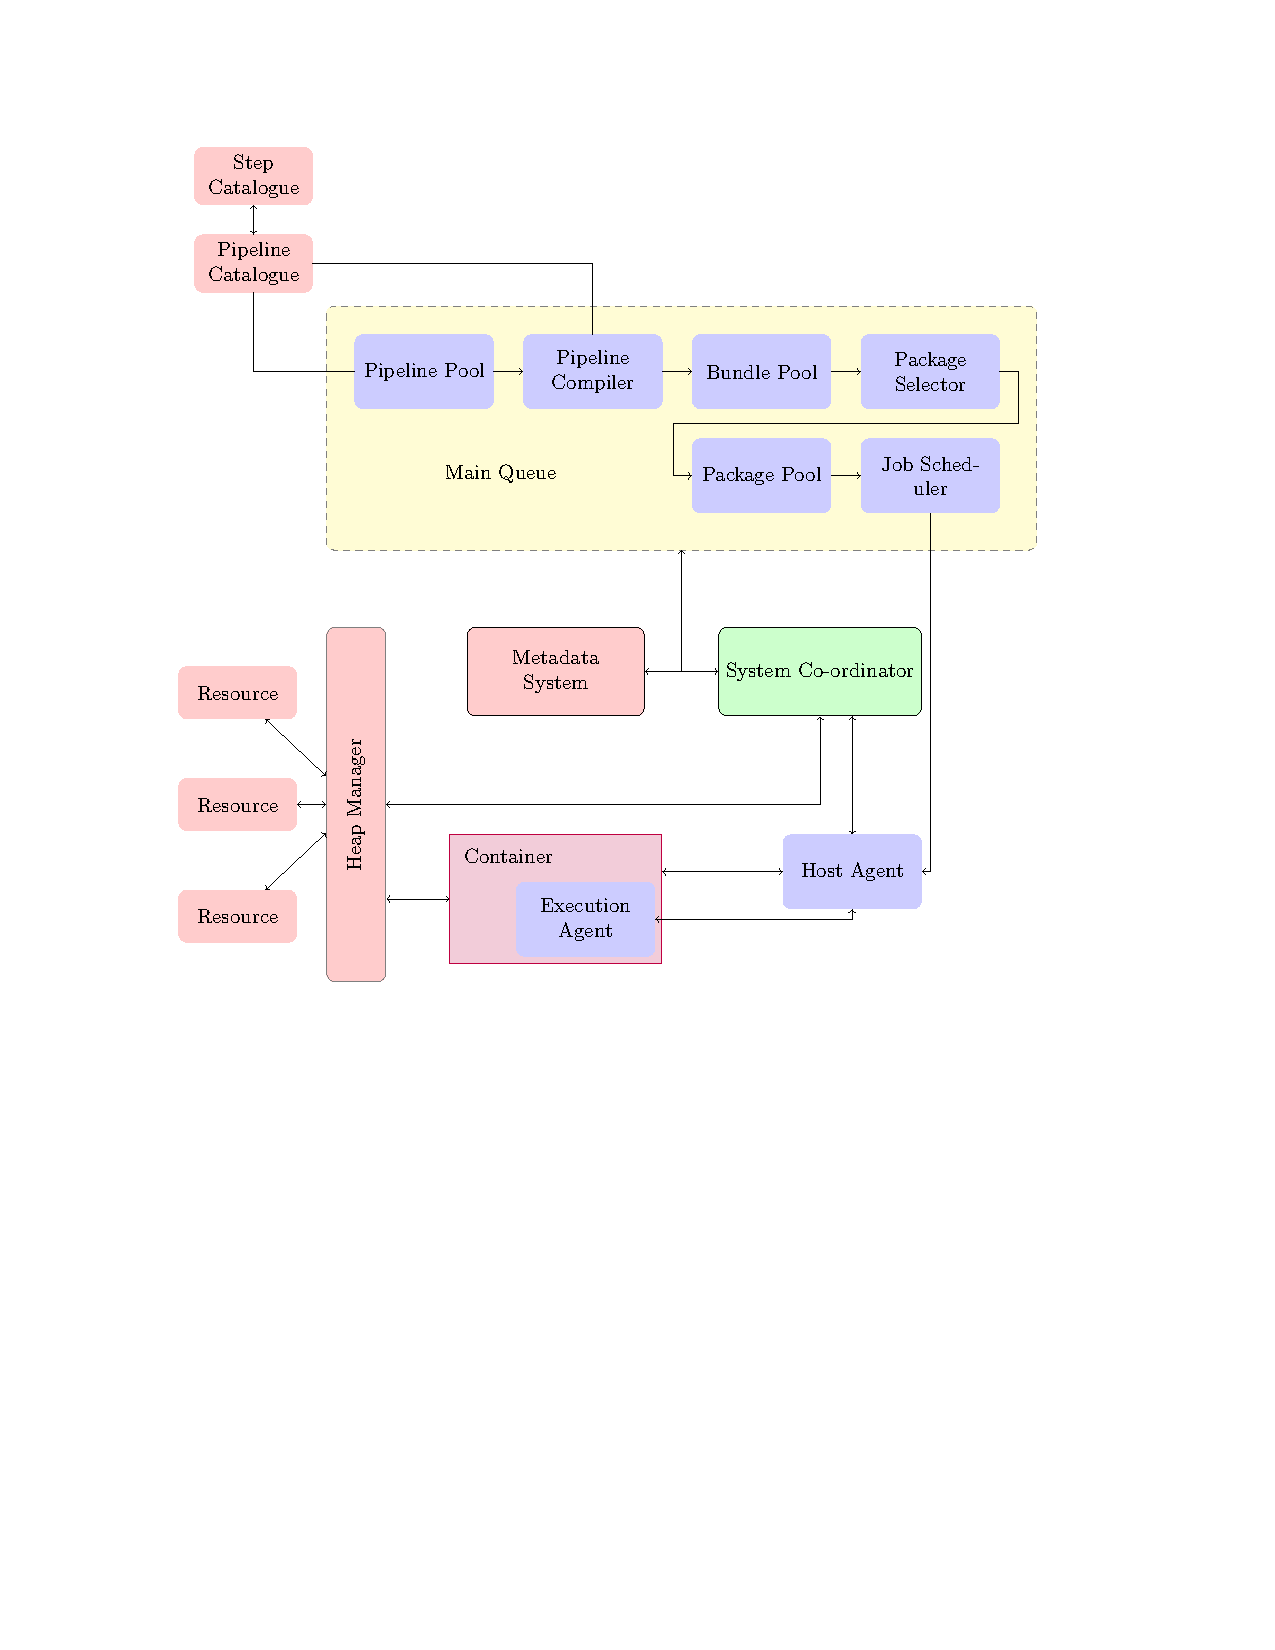
\includegraphics[height=0.85\paperheight]{images/mercury-system-diagram}
%		\hfil\hskip 2mm}\vfil}
%\end{backgroundblock}
%\end{frame}

%\section{\scshape Arvados}
%
%%%%%%%%%%%%%%%%%%%%%%%%%%%%%%%%%%%%%%%%%
%\subsection{Platform}
%\begin{frame}{Arvados Platform}
%\pipesbackground
%\shadedbackground{0.75}{1}
%\begin{backgroundblock}{0cm}{0cm}
%		\vbox to \paperheight{\vfil\hbox to \paperwidth{\hskip 6.5cm 
%		\begin{overpic}[height=0.85\paperheight]{images/Arvados-img01_-_cc-by-sa-4_0_-_Curoverse}
%		% Image source:https://arvados.org/images/img01.png
%		\put(57,-1){\textcolor{gray}{\fontsize{4}{6}\selectfont Curoverse, Inc.}}
%		\end{overpic}
%		\hfil\hskip 2mm}\vfil}
%\end{backgroundblock}
%\begin{itemize}
%\item Platform for data science
%\item Free \& open source (AGPL)
%\item Tracks provenance \\
%of data collections
%\item Allows jobs or whole \\
%pipelines to be repeated
%\item Jobs are isolated within \\
%Linux containers (docker)
%\item Data is deduplicated at block level
%\item Duplicate jobs are only run once
%\item Project-based security model for now
%\end{itemize}
%\end{frame}

%%%%%%%%%%%%%%%%%%%%%%%%%%%%%%%%%%%%%%%%
%\subsection{Technical Diagram}
%\begin{frame}{Technical Diagram}
%\pipesbackground
%\shadedbackground{0.5}{1}
%\begin{backgroundblock}{0cm}{0cm}
%		\vbox to \paperheight{\vfil\hbox to \paperwidth{\hskip 5.25cm 
%		\begin{overpic}[height=0.8\paperheight]{images/ArvadosTechnicalDiagramV16_website_-_cc-by-sa-4_0_-_Curoverse}
%		% Image source: https://dev.arvados.org/attachments/download/473/ArvadosTechnicalDiagramV16_website.png
%		\put(85,1){\textcolor{gray}{\fontsize{4}{6}\selectfont Curoverse, Inc.}}
%		\end{overpic}
%		\hfil\hskip 2mm}\vfil}
%\end{backgroundblock}
%\end{frame}

%%%%%%%%%%%%%%%%%%%%%%%%%%%%%%%%%%%%%%%%
%\subsection{Keep}
%\begin{frame}{Arvados Keep}
%\pipesbackground
%\shadedbackground{0.75}{1}
%\whitebackground{1}{0}{0.47}
%\begin{backgroundblock}{0cm}{0cm}
%		\vbox to \paperheight{\vfil\hbox to \paperwidth{\hskip 0.05\paperwidth 
%		\begin{overpic}[width=0.9\paperwidth]{images/Arvados-keep_workflow_diagram_2_-_cc-by-sa-4_0_-_Curoverse}
%		% Image source:https://dev.arvados.org/attachments/download/159/keep_workflow_diagram_2.png
%		\put(95,-1){\textcolor{gray}{\fontsize{4}{6}\selectfont Curoverse, Inc.}}
%		\end{overpic}
%		\hfil\hskip 2mm}\vfil}
%\end{backgroundblock}
%\end{frame}
%
%%%%%%%%%%%%%%%%%%%%%%%%%%%%%%%%%%%%%%%%%
%\subsection{Crunch}
%\begin{frame}{Arvados Crunch}
%\pipesbackground
%\shadedbackground{0.75}{1}
%\whitebackground{1}{0}{0.42}
%\begin{backgroundblock}{0cm}{0cm}
%		\vbox to \paperheight{\vfil\hbox to \paperwidth{\hskip 0.05\paperwidth 
%		\begin{overpic}[width=0.9\paperwidth]{images/Arvados-pipeline_workflow_diagram_1_-_cc-by-sa-4_0_-_Curoverse}
%		% Image source: https://dev.arvados.org/attachments/download/160/pipeline_workflow_diagram_1.png
%		\put(95,-1){\textcolor{gray}{\fontsize{4}{6}\selectfont Curoverse, Inc.}}
%		\end{overpic}
%		\hfil\hskip 2mm}\vfil}
%\end{backgroundblock}
%\end{frame}
%

%%%%%%%%%%%%%%%%%%%%%%%%%%%%%%%%%%%%%%%%
% Questions
%%%%%%%%%%%%%%%%%%%%%%%%%%%%%%%%%%%%%%%%
\section*{\scshape Questions}
\setbeamercolor*{background canvas}{bg=black}
\setbeamercolor{normal text}{fg=white, bg=black} 
\setbeamercolor*{structure}{fg=sangermidblue} 
\begin{frame}{Questions?}
\dcbackground
\end{frame}


\end{document}
